\documentclass{beamer}
%\documentclass[aspectratio=169]{beamer}  % inna proporcja slajdu

\usepackage[utf8]{inputenc}
\usepackage{polski}

\usepackage{graphicx}
\usepackage{multirow}
\usepackage{makecell}
\setcellgapes{5pt}

\usetheme{pwrlite}
%\usetheme[nosections]{pwrlite}  % wyłączenie stron z sekcjami
%\usetheme[en]{pwrlite}  % logo w wersji angielskiej
%\usetheme[nosections,en]{pwrlite}  % logo w wersji angielskiej i bez sekcji

%\pdfmapfile{+lato.map}  % jeśli nie działa font Lato (a jest zainstalowany), odkomentuj przy pierwszej kompilacji

\title{Wykrywanie oszustw na kartach płatniczych \\z~wykorzystaniem metod wrażliwych na koszt}
\institute{Promotor: dr inż. Andrzej Giniewicz \hfill Wydział Matematyki Politechniki Wrocławskiej}
\author{Patryk Wielopolski}

\begin{document}
	
	\newcommand{\htx}{h_{\theta}(\boldsymbol{x_i})}
	\newcommand{\es}{\mathcal{S}}
	\newcommand{\ef}{\mathcal{F}}
	\newcommand{\ku}{\mathcal{Q}}
	\newcommand{\iks}{\boldsymbol{x}}
	\newcommand{\yht}[1]{\hat{y_i}^{(#1)}}
	\newcommand{\ytrue}{\boldsymbol{y}}

\section{Wstęp}

\begin{frame}{Problem detekcji oszustw na kartach kredytowych}
	Zagadnienie:
	\begin{itemize}
		\item Detekcja nieautoryzowanych transakcji.
	\end{itemize}
	\pause
	
	Aktualna metodologia:
	\begin{itemize}
		\item Reguły eksperckie,
		\item Modele predykcyjne.
	\end{itemize}
	\pause
	
	Problem:
	\begin{itemize}
		\item Reguły eksperckie same nie wykrywają nowych zachowań przestępców.
		\item Standardowe modele predykcyjne nie biorą pod uwagę kosztu popełnienia błędu.
	\end{itemize}
	\pause
	
	Rozwiązanie:
	\begin{itemize}
		\item Modele predykcyjne wrażliwe na koszt.
	\end{itemize}
\end{frame}

\section{Część teoretyczna}

\begin{frame}{Miary skuteczności modeli}
	\begin{table}
		\begin{center}
			\begin{tabular}{c|c|c}
				\multirow{2}{8em}{} & Stan sprzyjający & Stan niesprzyjający \\
				& $y_i = 1$            & $y_i = 0$ \\
				\hline
				Predykcja pozytywna & \multirow{2}{8em}{\centering TP} & \multirow{2}{8em}{\centering FP} \\
				$c_i = 1$ &  &                 \\
				\hline
				Predykcja negatywna & \multirow{2}{8em}{\centering FN} & \multirow{2}{8em}{\centering TN} \\
				$c_i = 0$ &  &  \\
			\end{tabular}
		\end{center}
		\caption{Macierz pomyłek.}
		\label{tab:macierz-pomylek}
	\end{table}
	$$ \text{Precyzja} = \frac{TP}{TP + FP} $$ 
	$$ \text{Czułość}= \frac{TP}{TP + FN} $$
	$$ F_1 = \left(\frac{2}{\text{Precyzja}^{-1} + \text{Czułość}^{-1}}\right) $$
\end{frame}

\begin{frame}{Miary skuteczności modeli wrażliwych na koszt}
	\begin{table}
		\begin{center}
			\begin{tabular}{c|c|c}
				\multirow{2}{4em}{} & Stan pozytywny & Stan negatywny \\
				& $y_i = 1$            & $y_i = 0$ \\
				\hline
				Predykcja pozytywna & \multirow{2}{4em}{\centering $C^{(i)}_{1,1}$} & \multirow{2}{4em}{\centering $C^{(i)}_{1,0}$} \\
				$c_i = 1$         &                    &                    \\
				\hline
				Predykcja negatywna & \multirow{2}{4em}{\centering $C^{(i)}_{0,1}$} & \multirow{2}{4em}{\centering $C^{(i)}_{0,0}$} \\
				$c_i = 0$         &                    &                    \\
			\end{tabular}
		\end{center}
		\caption{Macierz kosztu dla $i$-tej obserwacji.}
		\label{tab:macierz-kosztu}
	\end{table}

	Oznaczenia:
	\begin{itemize}
		\item $\ytrue = (y_1, y_2, \dots, y_N)$ -- wektor prawdziwych stanów klasyfikacji,
		\item $\boldsymbol{c} = (c_1, c_2, \dots, c_N) $ -- wektor przewidywanych klas,
		\item $ \boldsymbol{C} = (C_1, C_2, \dots, C_N) $ -- wektor macierzy kosztu,
	\end{itemize}
\end{frame}

\begin{frame}{Miary skuteczności modeli wrażliwych na koszt}
	$$ \text{Oszczędności}(\ytrue, \boldsymbol{c}, \boldsymbol{C}) = \frac{\text{Koszt bazowy}(\ytrue, \boldsymbol{C}) - \text{TC}(\ytrue, \boldsymbol{c}, \boldsymbol{C})}{\text{Koszt bazowy}(\ytrue, \boldsymbol{C})} $$
	
	\vspace{0.7cm}
	Oznaczenia:
	\begin{itemize}
		\item $ \text{Koszt całkowity}(\ytrue, \boldsymbol{c}, \boldsymbol{C}) \text{ lub } \text{TC}(\ytrue, \boldsymbol{c}, \boldsymbol{C})= \sum_{i=1}^N C^{(i)}_{c_i,y_i} $
		\item $ \text{Koszt bazowy}(\ytrue, \boldsymbol{C}) = \min\{\text{TC}(\ytrue, \boldsymbol{c}_0, \boldsymbol{C}), \text{TC}(\ytrue, \boldsymbol{c}_1, \boldsymbol{C})\} \neq 0$
		\item $\boldsymbol{c}_0 = (0, 0, \dots, 0)$ -- $N$-elementowy wektor predykcji równych $0$,
		\item $\boldsymbol{c}_1 = (1, 1, \dots, 1)$ -- $N$-elementowy wektor predykcji równych $1$.

	\end{itemize}
\end{frame}

\begin{frame}{Modele predykcyjne}
	\begin{itemize}
		\item Standardowe modele predykcyjne:
		\begin{itemize}
			\item Regresja logistyczna
			\item Drzewo decyzyjne
			\item Las losowy
			\item XGBoost
		\end{itemize}
		\item Klasyfikacja wrażliwa na koszt:
		\begin{itemize}
			\item Minimalizacja ryzyka bayesowskiego
			\item Optymalizacja progu
		\end{itemize}
		\item Trening wrażliwy na koszt:
		\begin{itemize}
			\item Regresja logistyczna wrażliwa na koszt
			\item Drzewo decyzyjne wrażliwe na koszt
		\end{itemize}
	\end{itemize}
\end{frame}

\section{Eksperyment}

\begin{frame}{Zbiór danych}
	Wykorzystano zbiór danych \emph{Credit Card Fraud Detection}.
	\begin{itemize}
		\item Zawiera transakcje zawarte europejskimi kartami kredytowymi w~ciągu dwóch dni we wrześniu 2013 roku.
		\item Składa się z~284,807 transakcji, w~tym z~492 oszustw.
		\item Obserwacje są opisane 30 atrybutami, w~tym 28 z~nich to zanonimizowane zmienne numeryczne, które były wcześniej poddane transformacji PCA (\textit{ang. Principal Component Analysis}).
	\end{itemize}
\end{frame}

\begin{frame}{Metodologia eksperymentu}
	\begin{itemize}
		\item 50 powtórzeń symulacji Monte Carlo 
		\item Podział zbioru danych:
		\begin{itemize}
			\item 50\% zbiór treningowy
			\item 17\% zbiór walidacyjny
			\item 33\% zbiór testowy
		\end{itemize}
		\item Wykorzystane modele:
		\begin{itemize}
			\item Modele standardowe: regresja logistyczna, drzewo decyzyjne, las losowy, XGBoost
			\item Drzewo decyzyjne wrażliwe na koszt
			\item Optymalizacja progu oraz minimalizacja ryzyka bayesowskiego zastosowana dla modeli standardowych
		\end{itemize}
	\end{itemize}
\end{frame}

\begin{frame}{Wyniki dla oszczędności}
	\begin{figure}
		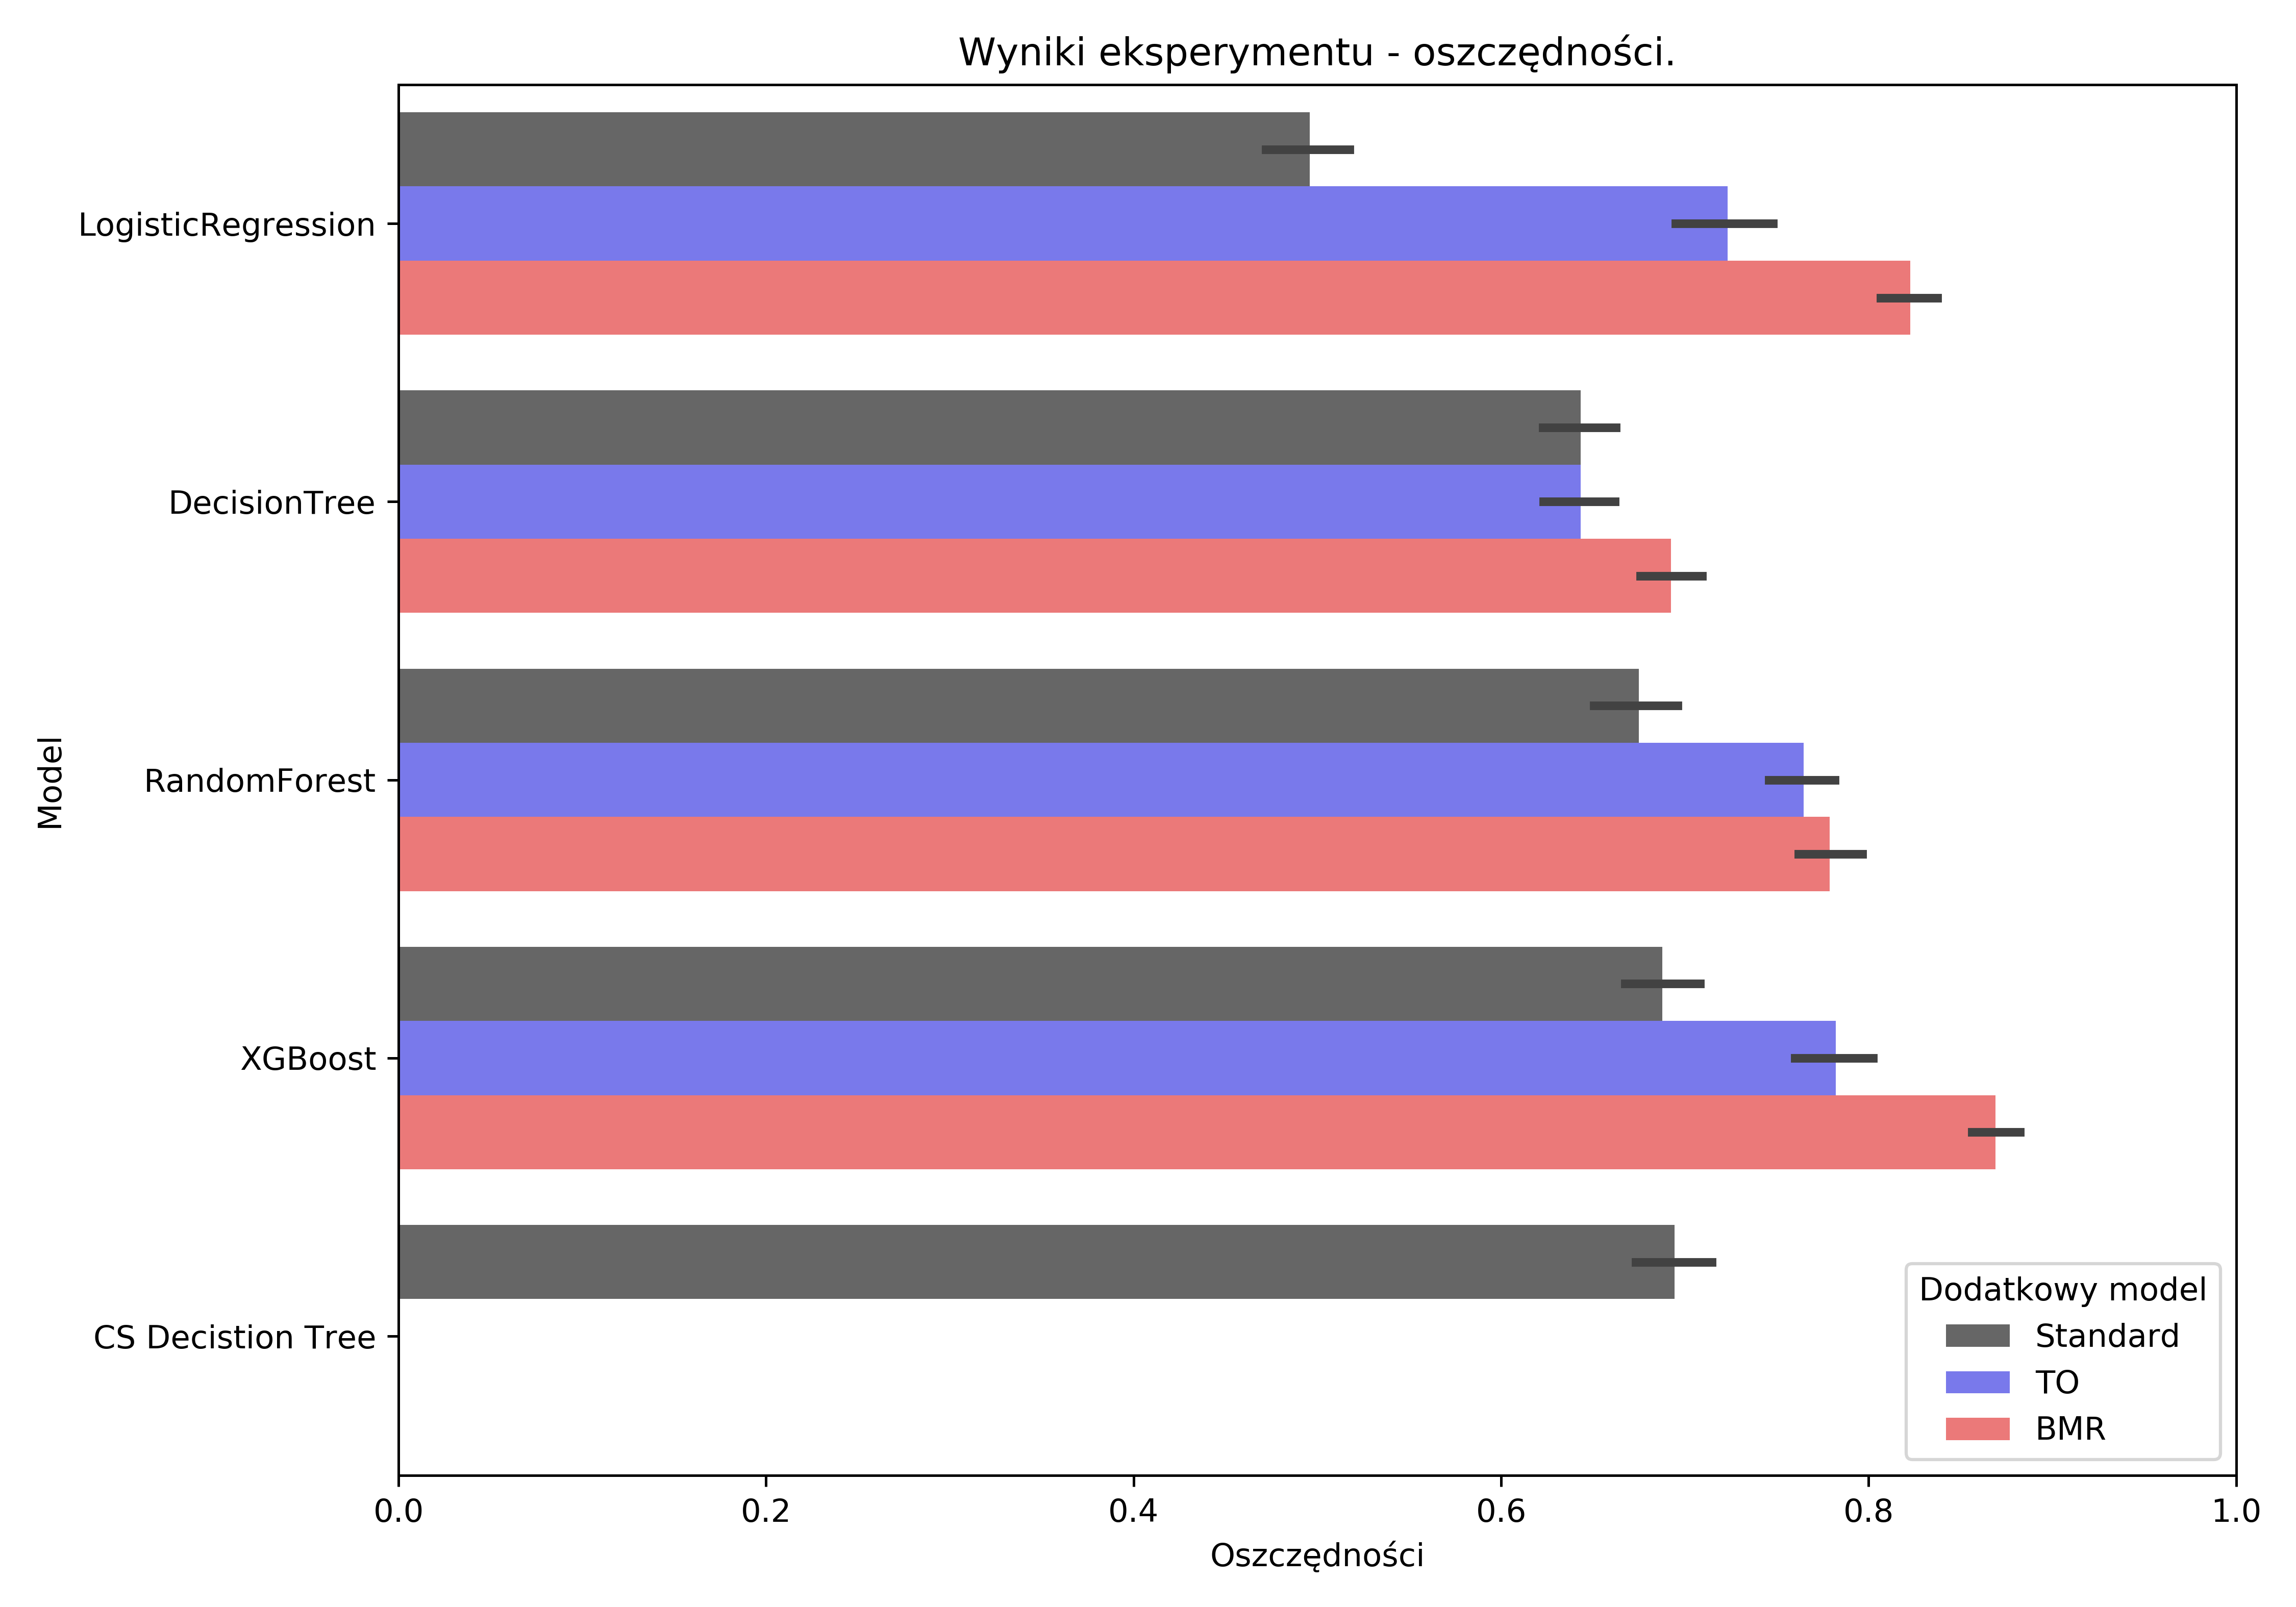
\includegraphics[width=0.8\linewidth]{images/100_config1-Savings.png}
		\caption{Wyniki eksperymentu dla oszczędności. Źródło: Opracowanie własne.}
	\end{figure}
\end{frame}

\begin{frame}{Wyniki dla F1 Score}
	\begin{figure}
		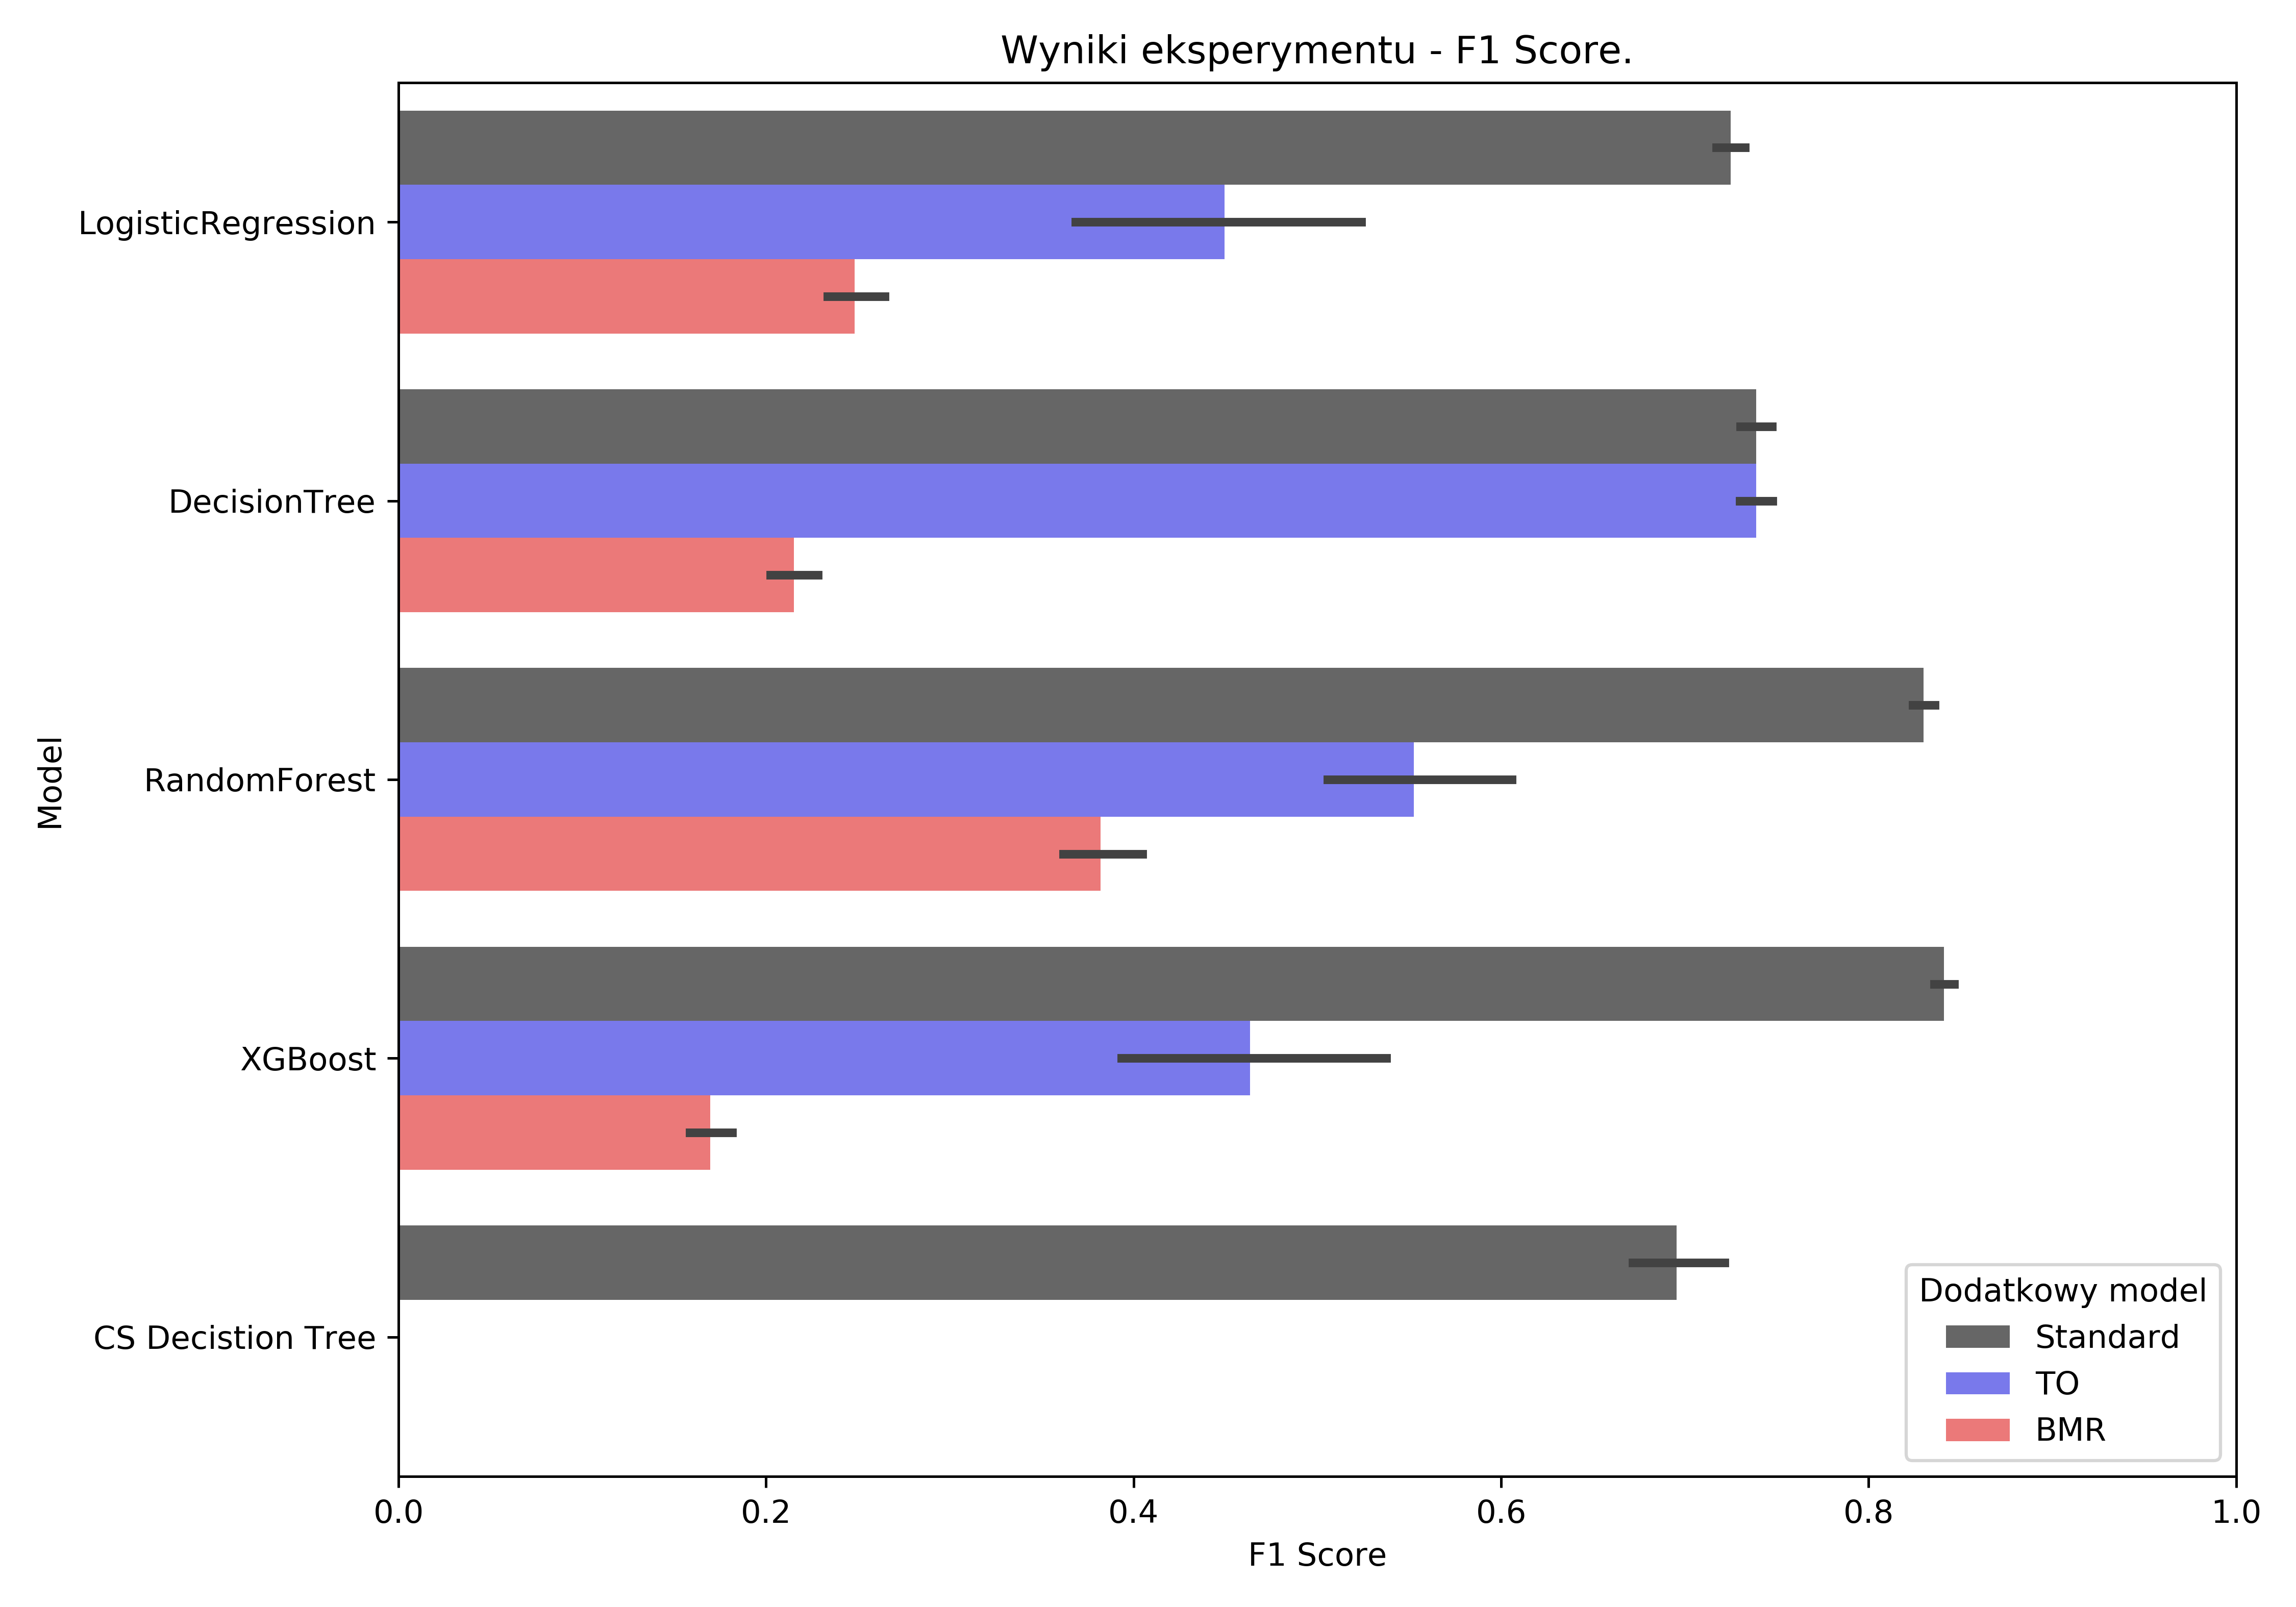
\includegraphics[width=0.8\linewidth]{images/100_config1-F1.png}
		\caption{Wyniki eksperymentu dla F1 Score. Źródło: Opracowanie własne.}
	\end{figure}
\end{frame}

\begin{frame}{Wnioski}
	\begin{itemize}
		\item Wykorzystanie metod wrażliwych na koszt pozwala na zwiększenie oszczędności. 
		\item Wykorzystanie powyższych metod obniża jakość predykcji w~kontekście standardowych miar skuteczności. 
		\item Drzewo decyzyjne wrażliwe na koszt uzyskuje zadowalające wyniki oszczędności, przy jednoczesnym zachowaniu wysokiej jakości predykcji w~kontekście standardowych miar skuteczności. 
	\end{itemize}
\end{frame}

\begin{frame}{Kierunek dalszych prac}
	\begin{itemize}
		\item Analiza metod typu ensemble z~drzewem decyzyjnym wrażliwym na koszt jako klasyfikator bazowy.
		\item Badania oraz implementacja algorytmu XGBoost z~drzewem decyzyjnym wrażliwym na koszt jako klasyfikator bazowy.
		\item Próba wykorzystania miary oszczędności jako niestandardowej funkcji kosztu w~algorytmie XGBoost.  
	\end{itemize}
\end{frame}

\begin{frame}{Bibliografia}
	\nocite{CSCCFD}
	\nocite{ICCFD}
	\nocite{EDCSLR}
	
	\bibliographystyle{bibliografia_styl}
	\bibliography{references}
\end{frame}

\section[]{Dziękuję za uwagę!}

\end{document}

